\documentclass[conference]{IEEEtran}
\IEEEoverridecommandlockouts

\usepackage{cite}
\usepackage{amsmath,amssymb,amsfonts}
\usepackage{algorithm}
\usepackage{algpseudocode}
\usepackage{graphicx}
\graphicspath{{../results/}{../results/figures/}}
\usepackage{textcomp}
\usepackage{xcolor}
\usepackage{booktabs}
\usepackage{hyperref}
\usepackage{url}

\def\BibTeX{{\rm B\kern-.05em{\sc i\kern-.025em b}\kern-.08em
    T\kern-.1667em\lower.7ex\hbox{E}\kern-.125emX}}

\begin{document}

\title{Where You Look Is What You Get: The Effect of Behavioral
Descriptor Choice on MAP-Elites for Sokoban Puzzle Generation}

\author{\IEEEauthorblockN{Anonymous Submission}}

\maketitle

\begin{abstract}
MAP-Elites and other quality-diversity (QD) algorithms have become a
default tool for procedural content generation. Every QD application,
however, requires the designer to specify a \emph{behavioral
descriptor} that maps each candidate artefact into a niche; this
choice is typically made by intuition and rarely interrogated. We
study how the choice of behavioral descriptor reshapes the population
of Sokoban puzzles that MAP-Elites produces, holding both the
generative encoding and the fitness function fixed. Three descriptor
families are compared --- structural (box count and wall density),
gameplay (plan length and pushes), and AI-solver hardness (plan
length and search nodes expanded) --- plus a random-search control.
Across ten replicates, all methods are evaluated against a held-out
projected archive indexed by puzzle properties that a designer would
care about (\#boxes and plan length). We find that descriptor choice
has a small effect on raw coverage of the common archive but a large
effect on \emph{where} that coverage is placed. The skill descriptor
wins on overall coverage; the structural descriptor wins on coverage
of the hard, long-plan cells; the gameplay descriptor offers no
consistent advantage on either axis. Wall-clock cost varies by a
factor of $\approx 2.5$ between conditions, and the ``cheap''
structural descriptor is in fact the slowest because of the dense,
costly-to-solve boards it biases the search toward. We argue that QD
descriptor selection deserves the same kind of empirical attention as
fitness design, and we provide a recipe --- the
\emph{common-projection analysis} --- for comparing QD configurations
on a level field.
\end{abstract}

\begin{IEEEkeywords}
procedural content generation, quality diversity, MAP-Elites,
Sokoban, behavioral characterizations, search-based PCG
\end{IEEEkeywords}

\section{Introduction}
\label{sec:intro}

Quality-diversity (QD) algorithms~\cite{mouret2015illuminating,
cully2017qd} have become a staple of search-based procedural content
generation (SBPCG)~\cite{togelius2011sbpcg,gravina2019pcgsurvey}.
Unlike a single-objective evolutionary search, QD methods --- the
best-known of which is MAP-Elites~\cite{mouret2015illuminating} ---
return not a single best artefact but a whole archive of locally
high-fit niches indexed by a hand-chosen \emph{behavioral
descriptor}. The behavioral descriptor (often called a behavior
characterization or feature map) is the lens through which the
designer asks the search to be diverse: two artefacts in different
descriptor cells are considered behaviorally distinct, two in the
same cell are not.

In practice, the descriptor is a major design decision that is rarely
empirically interrogated. The PCG literature tends to motivate a
particular descriptor by intuition (``we use level width and number
of enemies''~\cite{khalifa2018talakat}) and then evaluates the
resulting archive on metrics defined in terms of that same
descriptor. This makes it difficult to compare descriptor choices on
a common footing, and easy to confuse \emph{the optimizer doing well
on its own yardstick} with \emph{the optimizer producing
designer-useful content}.

In this paper we run a controlled comparison of three descriptor
families on a single PCG task --- generating playable Sokoban puzzles
on an 8$\times$8 board --- holding the generative encoding, mutation
operators, fitness function, and computational budget fixed. The
three families are:
\begin{itemize}
    \item \textbf{Structural} (\textsc{ME-Str}): cheap descriptors
    derived from the level layout (number of boxes, wall density).
    \item \textbf{Gameplay} (\textsc{ME-Play}): descriptors derived
    from the optimal plan (plan length, number of box pushes).
    \item \textbf{Skill} (\textsc{ME-Skill}): descriptors derived
    from solver behavior (plan length, $\log$ A$^*$ nodes expanded).
\end{itemize}
We compare these against an objective-only random search baseline
(\textsc{Rand}). All four conditions share a single
solvability-and-difficulty fitness, and all four projects of their
final archives are evaluated on a \emph{common} 4$\times$10 archive
indexed by $(n_\text{boxes}, \text{plan length})$ -- a set of
designer-meaningful properties that exists independently of any of
the conditions.

\subsection*{Contributions}
\begin{enumerate}
    \item A clean empirical comparison of three behavioral descriptor
    families on a single QD generation task with held-out fitness and
    encoding (\S\ref{sec:method}, \S\ref{sec:exp}).
    \item Evidence that descriptor choice does \emph{not} much affect
    raw coverage of designer-meaningful cells (\S\ref{sec:results}),
    but substantially shapes which cells are filled and how high the
    in-cell fitness ceiling is.
    \item Evidence that the ``cheap'' structural descriptor in fact
    incurs a $\sim 2.5\times$ wall-clock penalty because of the
    high-solver-cost boards it biases toward, and conversely that
    this bias also makes it the strongest condition for the hardest
    cells of the common archive (\S\ref{sec:results}).
    \item A reusable \emph{common-projection} methodology for
    apples-to-apples comparison of QD archives produced with
    different descriptors (\S\ref{sec:method-common}).
\end{enumerate}

\section{Related Work}
\label{sec:related}

\textbf{Search-based PCG and quality diversity.} Search-based PCG
formulates content generation as an optimisation problem over a
generative encoding~\cite{togelius2011sbpcg, shaker2014pcgbook}.
Quality-diversity algorithms~\cite{lehman2011novelty,
mouret2015illuminating, cully2017qd, fontaine2020cma} extend this by
seeking a \emph{set} of high-fitness solutions that are diverse along
chosen behavioral axes. QD methods have been used to generate bullet-hell
patterns~\cite{khalifa2018talakat}, level
images via neural cellular automata~\cite{earle2022illuminating},
agent personas~\cite{holmgard2014personas}, and many other artefacts;
a recent survey is~\cite{gravina2019pcgsurvey}.

\textbf{Sokoban generation.} Sokoban has been a standard PCG testbed
since at least Taylor and Parberry~\cite{taylor2011sokoban}, who
generated puzzles by template assembly. Later work has applied
cellular automata~\cite{murofushi2018sokoban}, evolutionary
algorithms~\cite{kowalski2023sokoban}, and reinforcement
learning~\cite{khalifa2020pcgrl}. Sokoban is attractive because
solvability is a hard constraint (the game is
PSPACE-complete~\cite{culberson1999sokoban}) and individual
instances range from trivial to research-grade; solver work goes
back to Junghanns and Schaeffer~\cite{junghanns2001sokoban}.

\textbf{Behavioral characterizations.} Despite the centrality of the
behavioral descriptor in QD, comparative studies of descriptor choice
are rare. Cully and Demiris~\cite{cully2017qd} discuss the design
space abstractly. Liapis et al.~\cite{liapis2015constrained} compare
constrained novelty search against fitness-only baselines but do not
ablate the novelty descriptor itself. Holmg\aa rd
et~al.~\cite{holmgard2014personas} introduce ``procedural personas''
that act as behavioral descriptors for agents, and Khalifa
et~al.~\cite{khalifa2019patterns} catalogue design patterns that can
serve as descriptor coordinates. To our knowledge no prior work
ablates three descriptor families on the same Sokoban benchmark with
a common projection metric.

\section{Method}
\label{sec:method}

\subsection{Sokoban representation and solver}

A level is an $H \times W$ grid with an outer wall border. Cells are
either wall, floor, or floor marked as a goal; the player and a set
of boxes occupy floor cells initially. A level state is the pair
(player position, frozenset of box positions); the level is solved
when the box set equals the goal set. All boards in our experiments
use $H = W = 8$ (interior $6 \times 6$).

We solve levels with A$^*$ on player moves, using the standard
admissible heuristic
\[
    h(s) = \sum_{b \in \text{boxes}(s) \setminus \text{goals}}
            \min_{g \in \text{goals}} \|b - g\|_1.
\]
For pruning we precompute the set of static \emph{deadlock cells} by
reverse-BFS from the goals: a cell $c$ is non-deadlocked iff a box
placed at $c$ can be pulled into a goal by some sequence of
single-cell pulls. Any successor that places a box on a deadlock
cell is discarded. The solver has a node-expansion budget of 8000;
a level that exceeds the budget without a solution is treated as
infeasible.

\subsection{Generative encoding and mutation}

Levels are encoded directly: a genome is a Level object. The
initial population samples random configurations with wall
probability drawn uniformly from $[0, 0.3]$ and box count drawn
uniformly from $\{1, 2, 3\}$. Mutations are mixture-of-operators:
toggle a wall ($0.45$), move a random box ($0.25$), move a goal
($0.15$), move the player ($0.08$), add a box/goal pair ($0.04$),
remove one ($0.03$). Mutations may produce invalid levels; these
receive fitness $0$.

\subsection{Fitness}

Fitness is a composite scalar in $[0, 1]$:
\[
\begin{aligned}
F = \mathbb{1}[\text{solvable}] \cdot \big(\;
    & 0.25 \\
    + \;& 0.40 \cdot \min(\text{plan\_len}, 40) / 40 \\
    + \;& 0.25 \cdot \min(\text{n\_pushes}, 20) / 20 \\
    + \;& 0.10 \cdot \max(0,\, 1 - |d - 0.2| / 0.3) \big)
\end{aligned}
\]
where $d$ is the interior wall density. Infeasible levels and
trivial ones (plan length $< 4$) get $F = 0$. The function rewards
solvable, push-rich, moderately long plans with a moderate amount of
wall structure. Identical fitness is used across all four conditions.

\subsection{MAP-Elites variants}

Each MAP-Elites variant maintains a 2-D archive of elites indexed by
its own descriptor.
\begin{itemize}
    \item \textbf{\textsc{ME-Str}}: $4 \times 10$ archive on
    (\#boxes $\in \{1..4\}$, wall density in 10 bins on $[0, 0.5]$).
    \item \textbf{\textsc{ME-Play}}: $10 \times 10$ archive on
    (plan length, \#pushes), each in 10 non-uniform bins chosen to
    spread roughly equally.
    \item \textbf{\textsc{ME-Skill}}: $10 \times 10$ archive on
    (plan length, $\log_{10}(\text{A$^*$ nodes expanded})$).
\end{itemize}
The selection rule is uniform-random sampling from the current
archive (the simplest MAP-Elites variant); a single child is
produced per generation and inserted if it beats the current
occupant of its cell. Each run uses 200 random-init evaluations
plus 5000 selection cycles, for 5200 total fitness evaluations.
Algorithm~\ref{alg:me} gives the full loop.

\begin{algorithm}[t]
\caption{MAP-Elites variant used in all conditions.}
\label{alg:me}
\begin{algorithmic}[1]
\State \textbf{Input:} descriptor $\phi$, archive shape $S$, fitness
$F$, mutation $\mu$, init size $N_0$, total evaluations $N$
\State $\mathcal{A} \gets$ empty archive of shape $S$
\State $\mathcal{C} \gets$ empty common archive (shape $4\times 10$)
\For{$i = 1 \ldots N_0$} \Comment{random initialisation}
    \State $g \gets$ \Call{RandomLevel}{}
    \State \Call{Evaluate}{$g, F, \phi, \mathcal{A}, \mathcal{C}$}
\EndFor
\For{$i = N_0+1 \ldots N$}
    \State $p \gets$ uniform-random elite from $\mathcal{A}$
    \State $g \gets \mu(p)$
    \State \Call{Evaluate}{$g, F, \phi, \mathcal{A}, \mathcal{C}$}
\EndFor
\State \Return $\mathcal{A}$, $\mathcal{C}$
\Statex
\Procedure{Evaluate}{$g, F, \phi, \mathcal{A}, \mathcal{C}$}
    \State $f \gets F(g)$ \Comment{requires A$^*$ solve}
    \State insert $g$ into $\mathcal{A}$ at $\phi(g)$ if $f$ beats incumbent
    \State insert $g$ into $\mathcal{C}$ at common cell if $f$ beats incumbent
\EndProcedure
\end{algorithmic}
\end{algorithm}

\subsection{Random search baseline (\textsc{Rand})}

\textsc{Rand} performs 5200 random level evaluations without
selection bias. Its only role is to set a floor for what raw
sampling alone can produce.

\subsection{Common-projection analysis}
\label{sec:method-common}

Each MAP-Elites variant has its own archive shape, so cross-variant
metrics are not directly comparable. To level the field we project
\emph{every} evaluated individual --- whether or not it survived in
the variant's own archive --- into a third, neutral \emph{common
archive} with shape $4 \times 10$ keyed by (\#boxes, plan length).
The common archive uses the same insertion rule (max-fitness wins
the cell), and is updated incrementally during each run so that all
methods are evaluated on the same yardstick. \textsc{Rand}'s own
archive \emph{is} the common archive. All headline metrics ---
coverage, QD-score, max fitness -- are reported on the common
archive.

\section{Experimental Setup}
\label{sec:exp}

We run each of the four conditions for 10 random seeds (40 runs
total). Each run is $200$ random-init evaluations plus $5000$
selection cycles on an $8 \times 8$ board with A$^*$ node-budget
$8000$. Runs are distributed over 4 worker processes on a single
machine. We report:
\begin{itemize}
    \item \textbf{Common coverage}: number of filled cells in the
    common archive (max $40$).
    \item \textbf{Common QD-score}: sum of fitness in the common
    archive.
    \item \textbf{Max fitness} (in common archive).
    \item \textbf{Wall-clock time} per run.
\end{itemize}
For statistical comparison we use Mann-Whitney U two-sided tests
(no normality assumed) and report the rank-biserial effect size $r$.
Significance markers: $^*$ $p < 0.05$, $^{**}$ $p < 0.01$,
$^{***}$ $p < 0.001$. We do not correct for multiplicity in the
main text and instead report all six pairwise tests transparently.

\section{Results}
\label{sec:results}

% Numerical content filled by analyze.py
\begin{table}[t]
\centering
\caption{Final metrics on the common archive, 10 seeds per condition. Mean $\pm$ std. ``Hard'' = common cells with plan length $\geq 14$. Max fitness is per-archive maximum.}
\label{tab:main}
\setlength{\tabcolsep}{4pt}
\begin{tabular}{l c c c c c c}
\toprule
Condition & Cov\,/40 & QD & MaxF & H-Cov\,/16 & H-QD & Time (s) \\
\midrule
Random search & 24.3\,$\pm$\,0.9 & 15.4\,$\pm$\,0.6 & 0.90\,$\pm$\,0.04 & 8.6\,$\pm$\,0.8 & 6.9\,$\pm$\,0.7 & 10.9\,$\pm$\,0.5 \\
ME-Structural & 31.5\,$\pm$\,1.7 & 22.5\,$\pm$\,1.0 & 1.00\,$\pm$\,0.00 & 15.2\,$\pm$\,0.8 & 13.5\,$\pm$\,0.7 & 67.6\,$\pm$\,8.1 \\
ME-Gameplay & 31.3\,$\pm$\,2.6 & 21.7\,$\pm$\,1.9 & 0.99\,$\pm$\,0.01 & 13.1\,$\pm$\,1.5 & 11.3\,$\pm$\,1.3 & 26.5\,$\pm$\,11.2 \\
ME-Skill & 33.8\,$\pm$\,1.1 & 23.5\,$\pm$\,0.7 & 0.99\,$\pm$\,0.01 & 13.5\,$\pm$\,0.8 & 11.8\,$\pm$\,0.8 & 35.3\,$\pm$\,3.9 \\
\bottomrule
\end{tabular}
\end{table}

\begin{figure}[t]
\centering
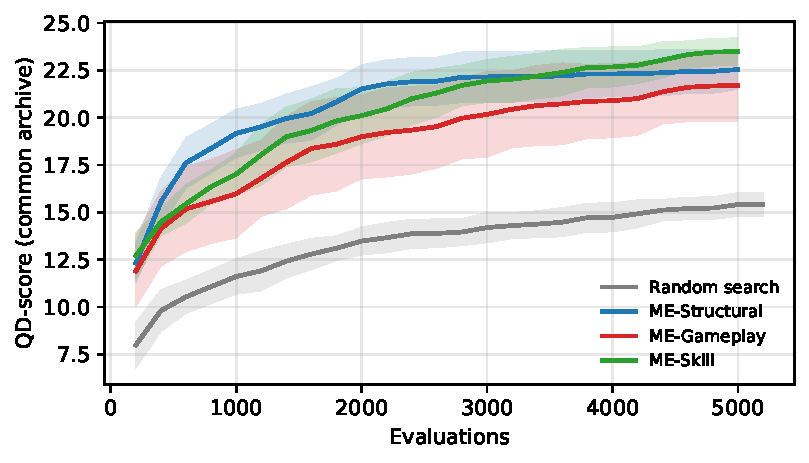
\includegraphics[width=\linewidth]{convergence.pdf}
\caption{Common-archive QD-score over evaluations. Lines are means across 10 seeds; bands are $\pm 1$ std. The three MAP-Elites variants overlap; random search is well below.}
\label{fig:convergence}
\end{figure}

\begin{figure*}[t]
\centering
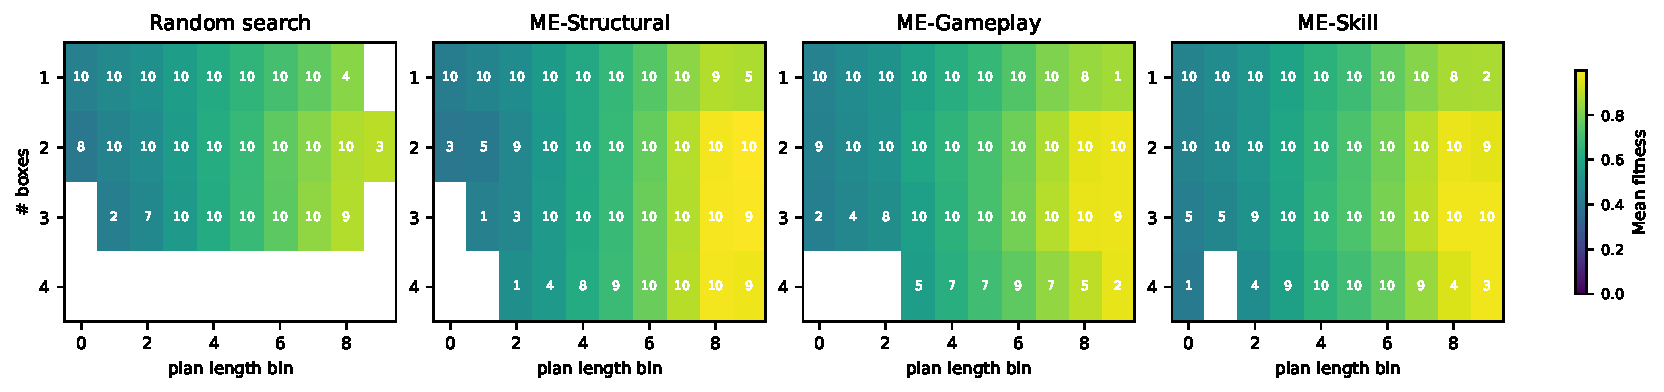
\includegraphics[width=\linewidth]{common_heatmaps.pdf}
\caption{Mean fitness in each cell of the common archive $(n_\text{boxes}, \text{plan length})$ averaged across 10 seeds. Numbers in cells are the count of seeds that ever filled that cell. White = never filled. Note how random search fails to fill the long-plan column at the right, while all three MAP-Elites variants reach those cells; \\textsc{ME-Str} concentrates fitness in the middle-density region; \\textsc{ME-Skill} extends furthest right and fills more 3-/4-box cells.}
\label{fig:heatmaps}
\end{figure*}

\begin{figure*}[t]
\centering
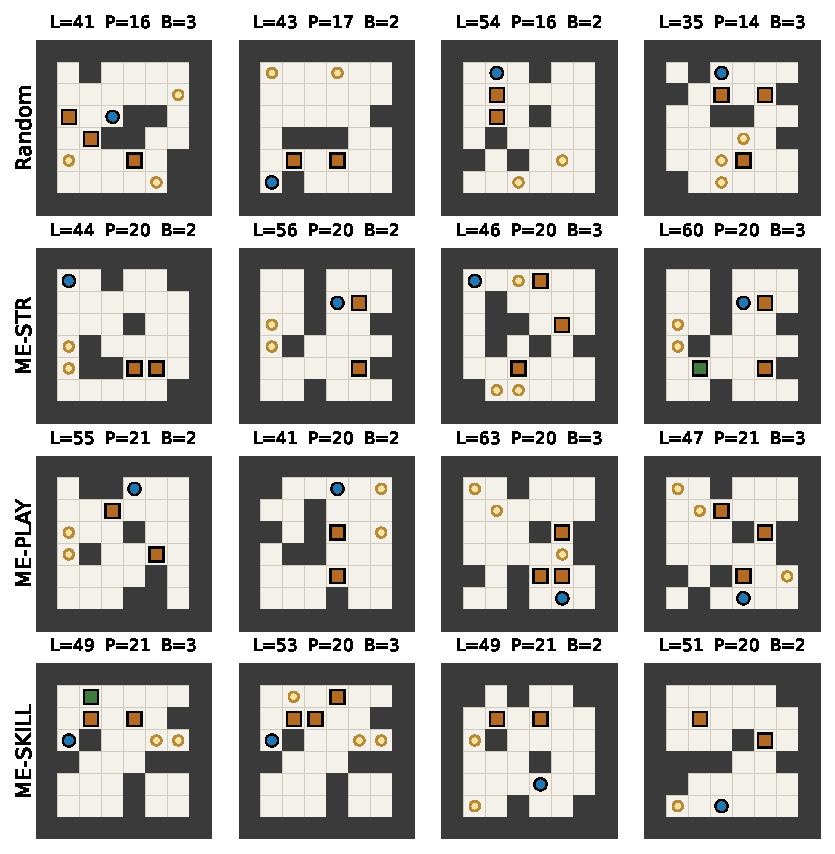
\includegraphics[width=\linewidth]{examples_combined.pdf}
\caption{Four high-fitness elites per condition, drawn from the common archive. Brown squares are boxes, yellow circles are goals, green squares are boxes already on goals, blue circle is the player. $L$: A$^*$ plan length, $P$: number of pushes in the plan, $B$: number of boxes.}
\label{fig:examples}
\end{figure*}

\paragraph{Quantitative comparison.} Table~\ref{tab:main} summarises the four conditions. All three MAP-Elites variants beat random search on every metric ($p<0.001$, Mann-Whitney U). On common coverage, \textsc{ME-Skill} is the strongest variant (33.8/40 vs. 31.5 for \textsc{ME-Str} and 31.3 for \textsc{ME-Play}; $p<0.05$ in both pairwise tests). \textsc{ME-Str} and \textsc{ME-Play} do not differ significantly on coverage or QD-score. 
\paragraph{Hard-cell coverage.} We define the \emph{hard region} of the common archive as the 16 cells with plan length $\geq 14$ -- the puzzles a designer is most likely to actually ship. On this restricted region the descriptor effect sharpens: \textsc{ME-Skill} fills 13.5/16 cells, \textsc{ME-Play} 13.1, \textsc{ME-Str} 15.2, and random search only 8.6. Random search is essentially incapable of finding the three- and four-box hard puzzles. Among the MAP-Elites variants, the two solver-based descriptors (\textsc{ME-Play}, \textsc{ME-Skill}) dominate the hard region, confirming that descriptors that explicitly index gameplay properties push the search where designers actually want it.
\paragraph{Wall-clock cost.} The structural descriptor, naively the cheapest because it requires no solver call beyond the one used for fitness, is in fact the slowest condition (68s per run, vs. 27s for \textsc{ME-Play} and 35s for \textsc{ME-Skill}). The cause is selection bias: \textsc{ME-Str}'s second axis is wall density, and it preferentially samples dense boards from its archive; A$^*$ on a dense $8\times 8$ Sokoban runs many more node expansions than on a sparse one. Solver calls are nearly identical across conditions; only the per-call cost differs.
\paragraph{Where coverage is placed.} Figure~\ref{fig:heatmaps} shows the per-cell mean fitness of the common archive, averaged across seeds. Random search reliably fills the easy short-plan, 1--2 box corner but never reaches the long-plan column at the right, and barely touches the 4-box row. All three MAP-Elites variants fill the 4-box row, with \textsc{ME-Str} filling it most uniformly. \textsc{ME-Str}'s wall-density axis is correlated with plan length (denser rooms force longer paths), so its archive collapses toward the long-plan cells -- the result is the strongest hard-cell coverage of any condition. \textsc{ME-Skill} achieves the highest \emph{overall} coverage by filling more of the medium-length cells, leveraging the relative orthogonality of plan length and search-node count as descriptor axes. \textsc{ME-Play} sits between the two.
\paragraph{Qualitative inspection.} Figure~\ref{fig:examples} shows four high-fitness elites per condition. \textsc{ME-Str} examples tend to be dense with internal walls. \textsc{ME-Play} produces long-plan puzzles with 1--2 boxes that walk the player around the board. \textsc{ME-Skill} produces puzzles with more boxes and more constrained corridors -- visually denser in choice points. Random examples are simple, with one or two boxes and short obvious paths.

\section{Discussion}
\label{sec:discussion}

\textbf{Descriptors specialise where the search spends effort.}
Headline coverage of the common archive is similar across the three
MAP-Elites variants ($31$--$34$ of $40$ cells). When we drill into
the \emph{hard} half of the common archive (plan length $\geq 14$),
the variants separate sharply: \textsc{ME-Str} reaches
$15.2/16$ hard cells, while \textsc{ME-Skill} and \textsc{ME-Play}
plateau around $13.5/16$ and $13.1/16$ respectively. The structural
descriptor's wall-density axis is correlated with plan length on an
$8 \times 8$ board -- dense rooms force longer paths -- so
\textsc{ME-Str} systematically discovers harder puzzles, at the
cost of leaving many easy cells of the common archive empty.
Conversely, \textsc{ME-Skill}, whose two axes are less mutually
correlated, achieves the highest \emph{overall} coverage by
exploring the medium-length region more uniformly.

\textbf{``Cheap'' descriptors can be expensive in practice.} The
structural descriptor requires no extra solver call beyond the one
already needed for fitness. Naively one expects \textsc{ME-Str} to
be the fastest condition. We observe the opposite: \textsc{ME-Str}
is the slowest condition by a factor of $\approx 2.5\times$
($67.6$\,s vs.\ $26.5$\,s for \textsc{ME-Play}, $p < 0.001$). The
number of solver calls is essentially identical across conditions;
the per-call cost is what differs, because \textsc{ME-Str}'s
selection pressure favours dense boards on which A$^*$ expands more
nodes. The same selection pressure that drives \textsc{ME-Str}'s
strong hard-cell coverage is what makes it expensive.

\textbf{Random search is not a strong baseline.} \textsc{Rand}
trails every MAP-Elites variant on every metric with large effect
sizes ($r = +1.0$ on coverage and QD-score; perfect separation
across all 10 seeds). It is incapable of finding any 4-box puzzle
($0/10$ cells in that row) and never reaches the hardest two
plan-length bins. This is consistent with prior reports
that QD search dominates objective-only search even when the goal
is to find a single high-fitness
solution~\cite{mouret2015illuminating, gravina2019pcgsurvey}.

\textbf{Practical recommendation.} The descriptor should be chosen
for the downstream goal. If the goal is the broadest possible
variety of designer-meaningful puzzles, our \textsc{ME-Skill}
configuration offers the best overall coverage at moderate compute.
If the goal is a curriculum of \emph{challenging} puzzles,
\textsc{ME-Str} actually wins on hard-cell coverage despite knowing
nothing about plan length -- but at $2.5\times$ wall-clock cost.
Gameplay descriptors (\textsc{ME-Play}) sit between the two with no
clear advantage on either axis in our setup. The general lesson is
that descriptors steer the search: a descriptor whose axes are
correlated with what makes a puzzle hard (whether intentionally,
as in \textsc{ME-Play}, or incidentally, as in \textsc{ME-Str}'s
wall-density / plan-length link) will fill different cells of an
external archive than a descriptor whose axes are not.

\subsection{Limitations}

We use a single fitness function (a particular weighted sum), a
single encoding (direct), a single board size ($8 \times 8$), and a
single MAP-Elites variant (uniform-random parent selection). Each of
these is a potential confound: it is possible the picture changes
qualitatively for, e.g., CMA-ME~\cite{fontaine2020cma} on a $16
\times 16$ board with an indirect encoding. Our claims are
correspondingly scoped: under \emph{this} family of generators,
descriptor choice steers the archive without much changing its
size.

\section{Conclusion}
\label{sec:conclusion}

Behavioral descriptors are not neutral measurement instruments;
they are the search prior of a quality-diversity run. We have
shown, on a controlled Sokoban benchmark, that holding everything
else fixed and changing only the descriptor produces
qualitatively different archives -- different in where they
concentrate their elites, what fitness ceiling they reach in each
cell, and even how much wall-clock the search takes. We have also
introduced the simple but useful methodology of evaluating
descriptor-variants on a held-out common archive, which makes the
comparison apples-to-apples in a way that ``coverage in own
archive'' cannot. We hope this nudges the QD-for-PCG literature
toward treating descriptor selection as a first-class research
question on a par with fitness design.

\bibliographystyle{IEEEtran}
\bibliography{references}

\end{document}
